\documentclass[a4paper,11pt,fleqn,dvipsnames,twoside,openright]{memoir} 	% Openright aabner kapitler paa hoejresider (openany begge)
\setlength{\paperheight}{297mm}
\setlength{\paperwidth}{210mm}
%%%% PACKAGES %%%%

% ¤¤ Oversaettelse og tegnsaetning ¤¤ %
\usepackage[utf8]{inputenc}					% Input-indkodning af tegnsaet (UTF8)
\usepackage[danish]{babel}					% Dokumentets sprog
\usepackage[T1]{fontenc}					% Output-indkodning af tegnsaet (T1)
\usepackage{ragged2e,anyfontsize}			% Justering af elementer
% \usepackage{fixltx2e}						% Retter forskellige fejl i LaTeX-kernen				
															
% ¤¤ Figurer og tabeller (floats) ¤¤ %
\usepackage{graphicx} 						% Haandtering af eksterne billeder (JPG, PNG, EPS, PDF)
%\usepackage{eso-pic}						% Tilfoej billedekommandoer paa hver side
%\usepackage{wrapfig}						% Indsaettelse af figurer omsvoebt af tekst. \begin{wrapfigure}{Placering}{Stoerrelse}
\usepackage{multirow}                		% Fletning af raekker og kolonner (\multicolumn og \multirow)
\usepackage{multicol}         	        	% Muliggoer output i spalter
\usepackage{rotating}						% Rotation af tekst med \begin{sideways}...\end{sideways}
\usepackage{colortbl} 						% Farver i tabeller (fx \columncolor og \rowcolor)
\usepackage{xcolor}							% Definer farver med \definecolor. Se mere: http://en.wikibooks.org/wiki/LaTeX/Colors
\usepackage{flafter}						% Soerger for at floats ikke optraeder i teksten foer deres reference
\let\newfloat\relax 						% Justering mellem float-pakken og memoir
\usepackage{float}							% Muliggoer eksakt placering af floats, f.eks. \begin{figure}[H]
\usepackage{longtable}
\usepackage[section]{placeins}

% ¤¤ Matematik mm. ¤¤
\usepackage{amsmath,amssymb,stmaryrd} 		% Avancerede matematik-udvidelser
\usepackage{mathtools}						% Andre matematik- og tegnudvidelser
\usepackage{textcomp}                 		% Symbol-udvidelser (f.eks. promille-tegn med \textperthousand )
\usepackage{rsphrase}						% Kemi-pakke til RS-saetninger, f.eks. \rsphrase{R1}
\usepackage[version=3]{mhchem} 				% Kemi-pakke til flot og let notation af formler, f.eks. \ce{Fe2O3}
\usepackage{siunitx}						% Flot og konsistent praesentation af tal og enheder med \si{enhed} og \SI{tal}{enhed}
\sisetup{output-decimal-marker = {,}}		% Opsaetning af \SI (DE for komma som decimalseparator) 

% ¤¤ Referencer og kilder ¤¤ %
\usepackage[danish]{varioref}				% Muliggoer bl.a. krydshenvisninger med sidetal (\vref)
\usepackage{natbib}							% Udvidelse med naturvidenskabelige citationsmodeller
%\usepackage{xr}							% Referencer til eksternt dokument med \externaldocument{<NAVN>}
%\usepackage{glossaries}					% Terminologi- eller symbolliste (se mere i Daleifs Latex-bog)

% ¤¤ Misc. ¤¤ %
\usepackage{listings}						% Placer kildekode i dokumentet med \begin{lstlisting}...\end{lstlisting}
\usepackage{lipsum}							% Dummy text \lipsum[..]
\usepackage[shortlabels]{enumitem}			% Muliggoer enkelt konfiguration af lister
\usepackage{pdfpages}						% Goer det muligt at inkludere pdf-dokumenter med kommandoen \includepdf[pages={x-y}]{fil.pdf}	
\pdfoptionpdfminorversion=6					% Muliggoer inkludering af pdf dokumenter, af version 1.6 og hoejere
\pretolerance=2500 							% Justering af afstand mellem ord (hoejt tal, mindre orddeling og mere luft mellem ord)

% Kommentarer og rettelser med \fxnote. Med 'final' i stedet for 'draft' udloeser hver note en error i den faerdige rapport.
\usepackage[footnote,draft,danish,silent,nomargin]{fixme}		

\usepackage{blindtext}
\usepackage{scrextend}
\addtokomafont{labelinglabel}{\textbf}

%%%% CUSTOM SETTINGS %%%%

% ¤¤ Marginer ¤¤ %
\setlrmarginsandblock{3.5cm}{2.5cm}{*}		% \setlrmarginsandblock{Indbinding}{Kant}{Ratio}
\setulmarginsandblock{2.5cm}{3.0cm}{*}		% \setulmarginsandblock{Top}{Bund}{Ratio}
\checkandfixthelayout 						% Oversaetter vaerdier til brug for andre pakker

%	¤¤ Afsnitsformatering ¤¤ %
\setlength{\parindent}{0mm}           		% Stoerrelse af indryk
\setlength{\parskip}{3mm}          			% Afstand mellem afsnit ved brug af double Enter
\linespread{1,1}							% Linie afstand

% ¤¤ Litteraturlisten ¤¤ %
\bibpunct[,]{[}{]}{;}{a}{,}{,} 				% Definerer de 6 parametre ved Harvard henvisning (bl.a. parantestype og seperatortegn)
\bibliographystyle{bibtex/harvard}			% Udseende af litteraturlisten.

% ¤¤ Indholdsfortegnelse ¤¤ %
\setsecnumdepth{subsection}		 			% Dybden af nummerede overkrifter (part/chapter/section/subsection)
\maxsecnumdepth{subsection}					% Dokumentklassens graense for nummereringsdybde
\settocdepth{subsection} 					% Dybden af indholdsfortegnelsen

% ¤¤ Lister ¤¤ %
\setlist{
  topsep=0pt,								% Vertikal afstand mellem tekst og listen
  itemsep=-1ex,								% Vertikal afstand mellem items
} 

% ¤¤ Visuelle referencer ¤¤ %
\usepackage[colorlinks]{hyperref}			% Danner klikbare referencer (hyperlinks) i dokumentet.
\hypersetup{colorlinks = true,				% Opsaetning af farvede hyperlinks (interne links, citeringer og URL)
    linkcolor = black,
    citecolor = black,
    urlcolor = black
}

% ¤¤ Opsaetning af figur- og tabeltekst ¤¤ %
\captionnamefont{\small\bfseries\itshape}	% Opsaetning af tekstdelen ('Figur' eller 'Tabel')
\captiontitlefont{\small}					% Opsaetning af nummerering
\captiondelim{. }							% Seperator mellem nummerering og figurtekst
\hangcaption								% Venstrejusterer flere-liniers figurtekst under hinanden
\captionwidth{\linewidth}					% Bredden af figurteksten
\setlength{\belowcaptionskip}{0pt}			% Afstand under figurteksten
		
% ¤¤ Opsaetning af listings ¤¤ %

\definecolor{commentGreen}{RGB}{34,139,24}
\definecolor{stringPurple}{RGB}{208,76,239}

\lstset{language=Matlab,					% Sprog
	basicstyle=\ttfamily\scriptsize,		% Opsaetning af teksten
	keywords={for,if,while,else,elseif,		% Noegleord at fremhaeve
			  end,break,return,case,
			  switch,function},
	keywordstyle=\color{blue},				% Opsaetning af noegleord
	commentstyle=\color{commentGreen},		% Opsaetning af kommentarer
	stringstyle=\color{stringPurple},		% Opsaetning af strenge
	showstringspaces=false,					% Mellemrum i strenge enten vist eller blanke
	numbers=left, numberstyle=\tiny,		% Linjenumre
	extendedchars=true, 					% Tillader specielle karakterer
	columns=flexible,						% Kolonnejustering
	breaklines, breakatwhitespace=true,		% Bryd lange linjer
}

% ¤¤ Navngivning ¤¤ %
\addto\captionsdanish{
	\renewcommand\appendixname{Appendiks}
	\renewcommand\contentsname{Indholdsfortegnelse}	
	\renewcommand\appendixpagename{Appendiks}
	\renewcommand\appendixtocname{Appendiks}
	\renewcommand\cftchaptername{\chaptername~}				% Skriver "Kapitel" foran kapitlerne i indholdsfortegnelsen
	\renewcommand\cftappendixname{\appendixname~}			% Skriver "Appendiks" foran appendiks i indholdsfortegnelsen
}

% ¤¤ Kapiteludssende ¤¤ %
\definecolor{numbercolor}{gray}{0.7}		% Definerer en farve til brug til kapiteludseende
\newif\ifchapternonum

\makechapterstyle{jenor}{					% Definerer kapiteludseende frem til ...
  \renewcommand\beforechapskip{0pt}
  \renewcommand\printchaptername{}
  \renewcommand\printchapternum{}
  \renewcommand\printchapternonum{\chapternonumtrue}
  \renewcommand\chaptitlefont{\fontfamily{pbk}\fontseries{db}\fontshape{n}\fontsize{25}{35}\selectfont\raggedleft}
  \renewcommand\chapnumfont{\fontfamily{pbk}\fontseries{m}\fontshape{n}\fontsize{1in}{0in}\selectfont\color{numbercolor}}
  \renewcommand\printchaptertitle[1]{%
    \noindent
    \ifchapternonum
    \begin{tabularx}{\textwidth}{X}
    {\let\\\newline\chaptitlefont ##1\par} 
    \end{tabularx}
    \par\vskip-2.5mm\hrule
    \else
    \begin{tabularx}{\textwidth}{Xl}
    {\parbox[b]{\linewidth}{\chaptitlefont ##1}} & \raisebox{-15pt}{\chapnumfont \thechapter}
    \end{tabularx}
    \par\vskip2mm\hrule
    \fi
  }
}											% ... her

\chapterstyle{jenor}						% Valg af kapiteludseende - Google 'memoir chapter styles' for alternativer

% ¤¤ Sidehoved ¤¤ %

\makepagestyle{IHA}							% Definerer sidehoved og sidefod udseende frem til ...
\makepsmarks{IHA}{%
	\createmark{chapter}{left}{shownumber}{}{. \ }
	\createmark{section}{right}{shownumber}{}{. \ }
	\createplainmark{toc}{both}{\contentsname}
	\createplainmark{lof}{both}{\listfigurename}
	\createplainmark{lot}{both}{\listtablename}
	\createplainmark{bib}{both}{\bibname}
	\createplainmark{index}{both}{\indexname}
	\createplainmark{glossary}{both}{\glossaryname}
}
\nouppercaseheads											% Ingen Caps oenskes

\makeevenhead{IHA}{Gruppe 1}{}{\leftmark}				% Definerer lige siders sidehoved (\makeevenhead{Navn}{Venstre}{Center}{Hoejre})
\makeoddhead{IHA}{\rightmark}{}{IHA - Aarhus Universitet}		% Definerer ulige siders sidehoved (\makeoddhead{Navn}{Venstre}{Center}{Hoejre})
\makeevenfoot{IHA}{\thepage}{}{}							% Definerer lige siders sidefod (\makeevenfoot{Navn}{Venstre}{Center}{Hoejre})
\makeoddfoot{IHA}{}{}{\thepage}								% Definerer ulige siders sidefod (\makeoddfoot{Navn}{Venstre}{Center}{Hoejre})
\makeheadrule{IHA}{\textwidth}{0.5pt}						% Tilfoejer en streg under sidehovedets indhold
\makefootrule{IHA}{\textwidth}{0.5pt}{1mm}					% Tilfoejer en streg under sidefodens indhold

\copypagestyle{IHAchap}{IHA}								% Sidehoved for kapitelsider defineres som standardsider, men med blank sidehoved
\makeoddhead{IHAchap}{}{}{}
\makeevenhead{IHAchap}{}{}{}
\makeheadrule{IHAchap}{\textwidth}{0pt}
\aliaspagestyle{chapter}{IHAchap}							% Den ny style vaelges til at gaelde for chapters
															% ... her
															
\pagestyle{IHA}												% Valg af sidehoved og sidefod


%%%% CUSTOM COMMANDS %%%%

% ¤¤ Billede hack ¤¤ %
\newcommand{\figur}[4]{
		\begin{figure}[H] \centering
			\includegraphics[width=#1\textwidth]{billeder/#2}
			\caption{#3}\label{#4}
		\end{figure} 
}

% ¤¤ Specielle tegn ¤¤ %
\newcommand{\decC}{^{\circ}\text{C}}
\newcommand{\dec}{^{\circ}}
\newcommand{\m}{\cdot}


%%%% ORDDELING %%%%

%%%% noget jesper har smidt ind %%%%
\hyphenation{}

\usepackage{graphicx}

\newcommand\xput[2][0.5]{%
    \rule{#1\linewidth}{0pt}\makebox[0pt][c]{#2}\hfill}

%%%% the end %%%%

\raggedbottom

\addbibresource{Referenceliste.bib}

\begin{document}


\includepdf{Filer/ProjektrapportForside.pdf}
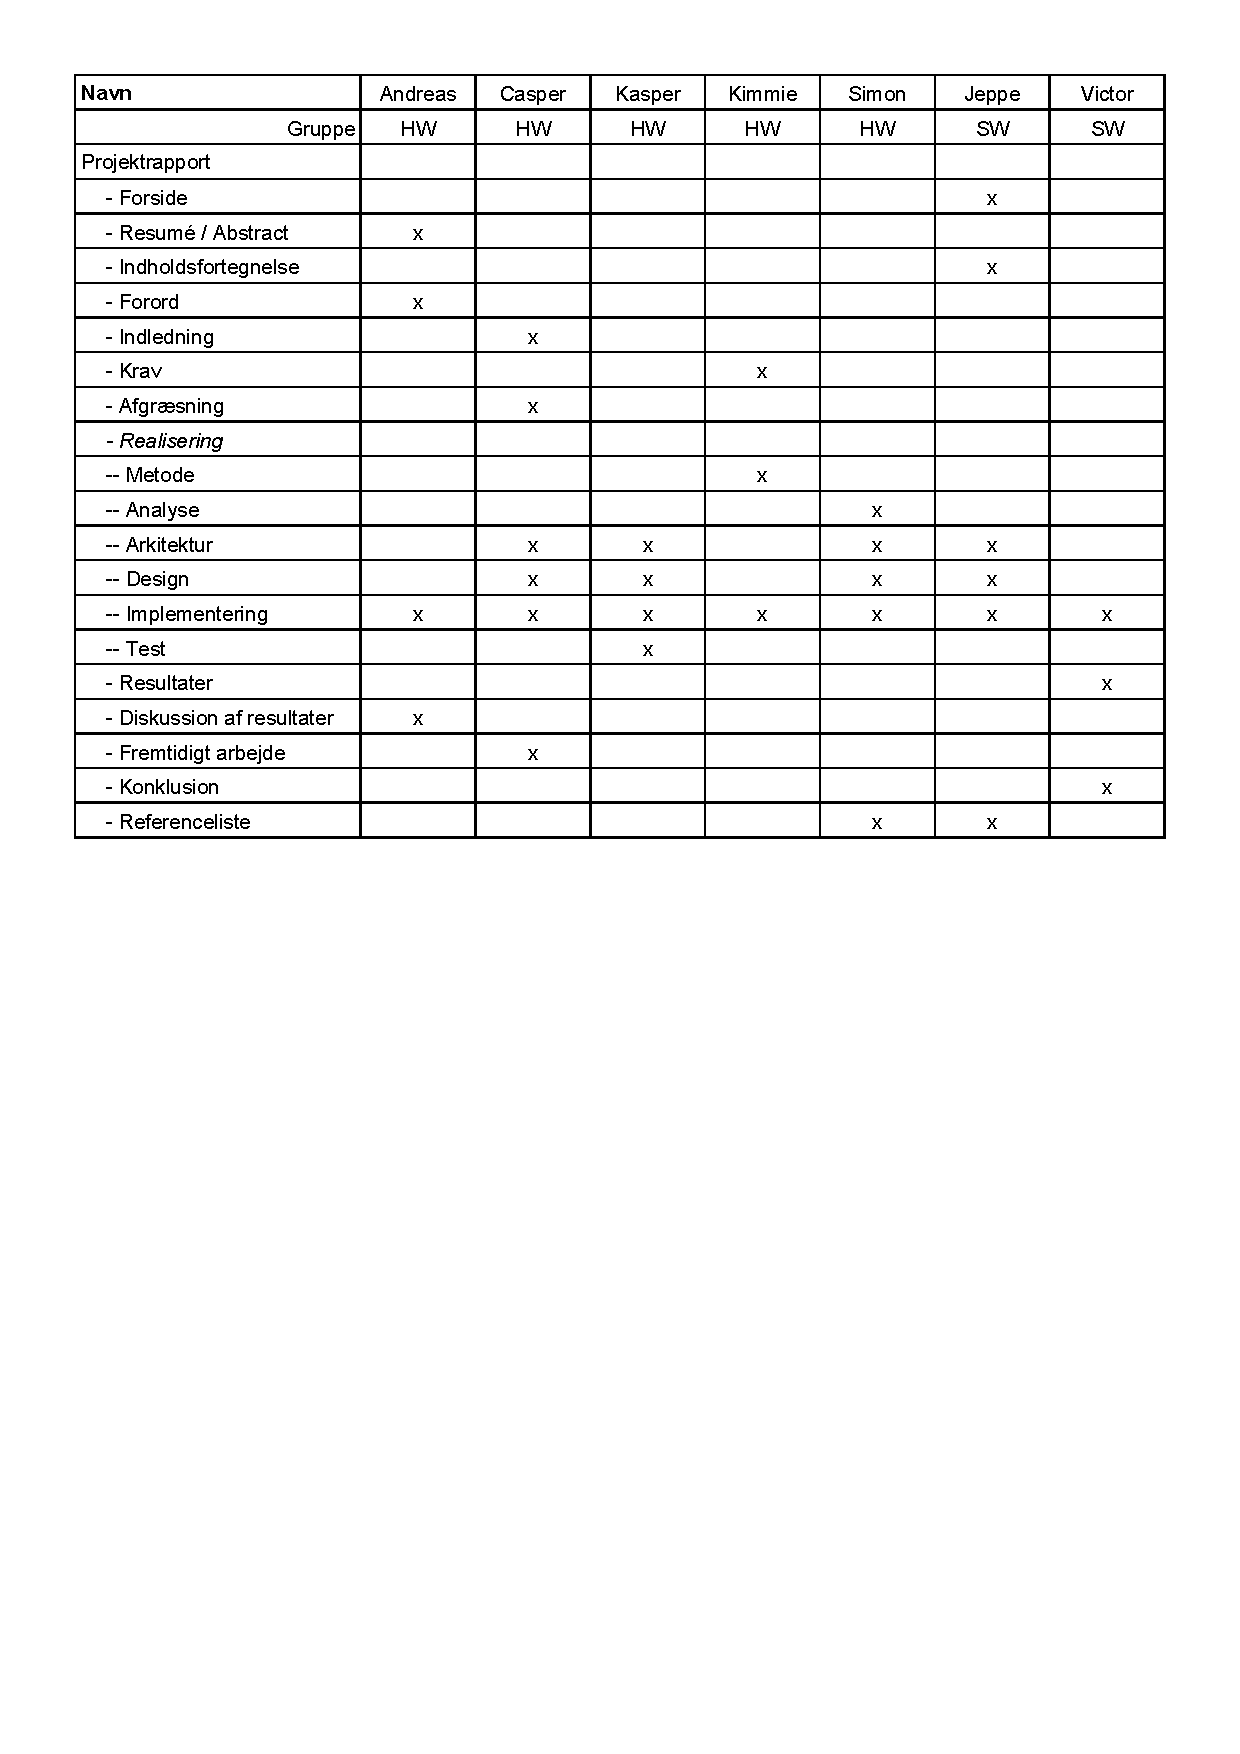
\includepdf{Filer/ProjektrapportArbejdsfordeling.pdf}

% 0. Resumé
% 0. Resumé / Abstract
\chapter*{Resumé / Abstract}

\section{Resumé}

Denne rapport beskriver udarbejdelsen af Gruppe 1’s projekt i forbindelse med kurset PRJ3 som er semmester-projektet på 3. semester på ASE. Projektet skulle indeholde aktuatorer, brugergrænseflade, faglige elementer fra andre fag, indlejret Linux- og en PSoC platform.

Den valgte projektformulering er at udvikle et automatisk lampe-hejsesystem ’L.A.M.P.’ der skal give mulighed for at finjustere en belysning. Dette hejse-system skal placeres under loftet i et lokale og skal styres fra en brugergrænseflade i form af en Devkit8000 touchkærm. Lampen skal kunne bevæge sig i 3 dimensioner: en X-akse og Y-akse (på langs og tværs af lokalet), samt en Z-akse (i højden). Lampen kan altså kunne placeres i en vilkårlig position i et hvert lokale. 3 typer sensorer skal derudover kunne detektere hhv. lysniveau i rummet, afstand fra lampe ned til nærmeste forhindring og om der er bevægelse i lokalet. 

Projektet er udført efter ASE-modellen og en prototype er blevet designet, konstrueret og implementeret. Projektets underemner, dvs. Projektformulering, Kravspecifikation, Design og Implementering er udarbejdet iterativt.

En række accepttest af funktionaliteten for L.A.M.P. er lavet og gennemført til at dokumentere at hele systemet er operativt og virker efter hensigten.

\section{Abstract}

This report describes the compiled project of Group 1 regarding the course PRJ3 which is the semester-project of the 3rd semester at ASE. The project was required to contain operators, a user interface, topics from other courses, embedded Linux and a PSoC platform.

The chosen project formulation is to develop an automatic lamp-crane-system ‘L.A.M.P.’ that will enable the lamps position to be easily customized. The crane-structure will be placed under the ceiling in a room and will be controlled from an accessible user interface by means of a Devkit8000 touchscreen. The lamp will be able to be moved in 3 dimensions: An X- and Y-axis (along and across the room) and a Z-axis (at height). The lamp is able to be positioned freely in a limited 3-dimensional space. 3 different types of sensors will also respectively detect the brightness in the room, the distance from the lamp down to nearest obstacle and whether there is any movement in the room or not.

The Project is completed trough the ASE-model and a prototype has been designed, constructed and implemented. The subtopics of the project, that is, Project formulation, Requirements-specifications, design and implementation are created iteratively.

A series of Acceptance-tests of the functionality for L.A.M.P is conducted and completed in order to ensure the total system is operational and works as intended.


% 0. Abstract
% 0. Abstract
\chapter*{Abstract}

This report describes the compiled project of Group 1 regarding the course PRJ3 which is the semester-project of the 3rd semester at ASE. The project was required to contain operators, a user interface, topics from other courses, embedded Linux and a PSoC platform.

The chosen project formulation is to develop an automatic lamp-crane-system ‘L.A.M.P.’ that will enable the lamps position to be easily customized. The crane-structure will be placed under the ceiling in a room and will be controlled from an accessible user interface by means of a Devkit8000 touchscreen. The lamp will be able to be moved in 3 dimensions: An X- and Y-axis (along and across the room) and a Z-axis (at height). The lamp is able to be positioned freely in a limited 3-dimensional space. 3 different types of sensors will also respectively detect the brightness in the room, the distance from the lamp down to nearest obstacle and whether there is any movement in the room or not.

The Project is completed trough the ASE-model and a prototype has been designed, constructed and implemented. The subtopics of the project, that is, Project formulation, Requirements-specifications, design and implementation are created iteratively.

A series of Acceptance-tests of the functionality for L.A.M.P is conducted and completed in order to ensure the total system is operational and works as intended.

% 1. Ordliste
\chapter{Ordliste}

\begin{description}
    \item [Basen] Objekt som Lampen er monteret på. Lampen hejses ned fra denne i Z-aksen.
    \item [Bevægelsessensor] Ultra Sonic sensor der detekterer bevægelse i rummet.
    \item [Devkit8000] Embedded Linux platform udleveret i forbindelse med fagene HAL og ISU.
    \item [GUI] Det grafiske brugerinterface på Devkit8000 touchskærmen.
    \item [L.A.M.P] Det samlede system der skal udvikles.
    \item [PSoC] Programmable System on Chip.
    \item [PSoC-Master] 
    \item [PSoc-Sensor] 
    \item [PSoC-XY] 
    \item [PSoC-Z] 
    \item [Pile-kryds] 4 pil-knapper der sidder på GUI, som peger hhv. peger op,ned, til venstre og til højre.
    \item [“Rød/Grøn/Blå farve”-slider] Virtuelle sliders på GUI’en som lader en bruger justere farven.
    \item [Sideskinner] 2 skinner som sidder i hver side af loftet. Tværskinnen sidder mellem disse til bevgægelse i X-asken.
    \item [Touchskærm] Den touch følsomme skærm på Devkit8000.
    \item [Tværskinne] Skinne der kan føres frem og tilbage i loftet. Basen sider på denne skinne til bevægelse i Y-aksen.
    \item ["X, Y, Z"-slider] Virtuelle sliders på GUI'en som justere for position af lampen i tre akser.
    \item [U.S.] Se: Bevægelsessensor.
\end{description}

\tableofcontents*
\clearpage

\listoffigures
\clearpage

% 1. Forord
% 1. Forord
\chapter{Forord}

Under semesterprojekt 3 for tredje semester på ingeniørhøjskolen i Århus består gruppe 1 af 2 IKT-, 3 E- og 2 EP-studerende. 
Projektet skal afleveres d. 27. maj og bedømmes d. 21. juni.
Vores materiale dokumenteres med en projektrapport, en dokumentationsrapport, bilag og denne processrapport.

% 2. Indledning
% 2. Indledning
\chapter{Indledning}

Udviklingsprocessen har gennem dette semester fungeret i et jævnt flow. Vores første projektgruppemøde bestod af en præsentationsrunde. Vi forklarede lidt om hvem vi hver især var, og hvad vi prioriterer i et projektarbejde, og lærte hinanden bedre at kende. Vores andet møde var et brainstorm møde, hvor vi skulle lægge os fast på hvilket produkt der skulle laves. Vi blev enige om et af de mange forslag, og har siden arbejdet målrettet for at realisere dette produkt.

Vi lavede en arbejdsopgavetavle som var meget Scrum-inspireret(Se figur \ref{fig:SB})\footcite{scrum}, og satte alle vores opgaver på denne med tegnestifter. 
Vi har i processen været fælles omkring struktureringen. Dvs man flyttede selv sine opgaver fra ”In progress” til ”Done” på vores projektopgavetavle, skrev selv tilføjelser til dagsordener og hjalp til med strukturering af filer i projektmapper. 
Enkelte områder fik en fast tovholder. Vi fordelte disse poster ud som følger:

\begin{table}[H] \centering
\begin{tabular}{|r|r|}
	\hline
		Jeppe & Ordstyrer ved møder \\ \hline
		Casper & Ordstyrer ved møder \\ \hline
		Victor & Referrent ved projektmøder \\ \hline
		Kimmie & Kageordning ved projektmøder \\ \hline
	\end{tabular}
\end{table}

% 3. Krav
% 3. Krav
\chapter{Krav}

Projektets aktører er brugeren, bevægelse i rummet og fysiske objekter under lampen. Brugeren er den primære aktør, og den der interagerer aktivt med produktet. Både bevægelse og fysiske objekter er sekundære aktører. Begge disse er sat som aktører da de aktiverer funktionalitet i produktet. Bevægelse registreres af en sensor, hvorefter lyset tændes. Fysiske objekter under lampen aktiverer, at lampen stopper nedadgående bevægelse, hvis lampen kommer for langt ned.
Vi har i projektet 5 Usecases (UC). De hedder følgende:

\begin{itemize}
    \item UC1: Kalibrér system.
    \item UC2: Tænd/Sluk lys.
    \item UC3: Registrér bevægelse.
    \item UC4: Juster lysets farve.
    \item UC5: indstil placering af lampen.
\end{itemize}

I UC1 kan brugeren, via systemets GUI, vælge at kalibrere systemet. Dette nulstiller lampens position i rummet, og gør efterfølgende placering af lampen mere præcis.

I UC2 kan brugeren, via systemets GUI, tænde og slukke for lampen. Dette gøres ved et simpelt tryk på en knap på touchskærmen.

I UC3 kan brugeren, via systemets GUI, aktivere funktionen ”registrér bevægelse”. Når denne funktion er aktiv, vil bevægelse i rummet resultere i at lyset tændes.

I UC4 kan brugeren, via systemets GUI, ændre på lysets farvetone. Dette gøres ved at indstille mængden af rødt, grønt og blåt lys lampen afgiver. Dette har også indvirkning på lysstyrken, da en kraftigere mængde af en eller flere farver vil give større lysstyrke.

I UC5 kan brugeren, via systemets GUI, vælge hvor i rummet lampen skal placeres. Dette sker ved at flytte på en slider for hhv. X, Y og Z aksen, og dermed indstille en position for lampen i alle bevægelses retningerne.

Alle aktører og Usecases inkl. tilhørende diagrammer, kan findes i dokumentationsrapporten\footcite{documentation} under punkt 2.2 Usecases.

Projektet er planlagt med en række ikke funktionelle krav inddelt under Usability, Reliability, Performance, Supportability og generelle krav. De ikke funktionelle krav definerer under disse emner, systemets minimums levetid uden nedbrud og software’ens oppetid uden genstart. Derudover defineres betjeningsvenligheden, systemets responstid og almindelig vedligehold. De generelle krav fortæller hvad vægt tolerancen er for lampen, og hvad spændingstilslutning systemet kræver. Detaljerne kan findes i dokumentationsrapporten\footcite{documentation} under punkt 2.4 Ikke-funktionelle krav. 


% 4. Afgrænsning
% 4. Afgrænsning
\chapter{Afgrænsning}

Når projektets use cases og funktionalitet er beskrevet, kan hardwareelementerne der skal implementeres fastlægges. Det er nødvendigt at have en fyldestgørende beskrivelse for de funktioner produktet skal kunne opfylde og udføre for at vælge de bedst mulige komponenter til at gennemføre dette. Grundet tidsrammen for projektet er det nødvendigt at begrænse sig for funktionalitet. Derfor vil det også være nødvendigt at fravælge nogle af de overvejede komponenter. Overvejelserne går på hvad der er vigtigst for produktets minimumsfunktionalitet.
Følgende produkter kunne implementeres i det endelige produkt:

\textbf{Kontakt (Tilvalgt)}
For at vognene i systemet ikke skulle køre ud over deres skinner er det nødvendigt at detektere skinnernes yderste position. Dette gøres ved en fysisk kontakt som slutter når vognen er i yderposition i enten X- eller Y-aksen. Derfor var en Kontakt nødvendig at have med. 

\textbf{Afstandssensor (Tilvalgt)}
For at vores lampe ville være i stand til at detektere sin bundposition var en form for sensor nødvendig at implementere her også. En afstandssensor ville være mere alsidig og give flere muligheder end en kontakt der blev monteret i lampeskærmen. Derfor blev afstandssensoren implementeret i produktet.

\textbf{Bevægelsessensor (Tilvalgt)}
I stedet for at tænde systemets lys med en kontakt, blev det valgt at en bevægelsessensor skulle benyttes. Blandt andet fordi endnu en kontakt ikke ville være en udfordring, fordi der skulle trækkes flere løse ledninger og fordi udfordringen at arbejde med bevægelsessensoren var størst, blev denne sensor valgt.

\textbf{Lumensensor (Tilvalgt)}
For at give produktet funktionaliteten at automatisk kunne justere lysforholdene i rummet, måtte en lumensensor implementeres. Dette for blandt andet at kunne sætte et skema op for hvornår lyset skulle tændes eller ikke tændes, f.eks om morgenen i forhold til sommer-/vintertid. Desværre var produktets LED’er ikke kraftige nok til at give et på lumensensoren målbart arbejdsområde, så lumensensoren er ikke fuldt ud implementeret.

\textbf{Farvetemperatursensor (fravalgt)}
For at give produktet en ekstra feature der er en smule mere detaljeret end en almindelig lyssensor, var det muligt at implementere en farvetemperatursensor. At måle lysniveauer i rødt, grønt, og blåt lys fremfor blot at måle på hvidt lys ville være en forbedring af produktet da det nu også ville være et salgsargument for personer med visse øjensygdomme eller særlig følsomhed for bestemte lysspektre. Denne sensor blev fravalgt da den krævede et filter for at kunne måle det menneskelige synlige spektre. Uden dette filter målte den også infrarøde lysværdier. Grundet tidsrammen for projektet var der for meget arbejde i denne sensor, og den blev derfor fravalgt.  

\textbf{Trådløs styring (fravalgt)}
Produktet kunne udvides med trådløs betjeningspanel. Dette ville frigøre brugeren for at skulle tænke over hvor vedkommende skulle montere sit Devkit8000 i rummet. Da dette bliver betragtet som en feature der er unødvendig for produktets egentlige funktion, samt projektets tidsramme, blev denne funktionalitet fravalgt.  

\textbf{Gsm-modul (fravalgt)}
Lignende trådløs styring, kunne produktet styres trådløst via mobiltelefon. Dette ville frigøre nødvendigheden af et Devkit8000 og gøre brugeren i stand til at styrer produktet uanset hvor han er, så længe det er inden for mobildækning. Dette blev også fravalgt grundet unødvendighed og tidsramme. 



% 5. Realisering
% 4. Realisering
\chapter{Realisering}


% 4.1 Metode
\section{Metode}

Til beskrivelse af software er der brugt UML og 4+1 modellen. Til de grafiske beskrivelser af systemet, både opbygningsmæssigt og funktionsmæssigt, er der blevet brugt SysML.

UML står for Unified Modelling Language, diagramtyperne i UML kan deles op i to grupper: strukturdiagrammer og adfærdsdiagrammer. Det er ved hjælp af diagrammer at alle klasse diagrammer, sekvensdiagrammer o. lign. er lavet. Ulempen ved UML i forhold til resten af projektet, er at det er meget software centreret, og dermed mindre velegnet til beskrivelse af resten af projektet. 

4+1 modellen er en view model designet til at beskrive software tunge systemer fra de forskellige stakeholder perspektiver. Modellen er brugt til at lave logic view, deployment view, implementation view og data view. Valget faldt på denne model, da systems kompleksitet i forhold til software blevet uoverskueligt lavet ved hjælp af UML diagrammer.

SysML står for System Modelling Language og er en udvidelse af UML, lavet med fokus på hardware og generelle system beskrivelser. SysML er brugt til at lave BDD’er, IBD’er Use Case diagrammer med mere, men ikke til softwaren. Dette skyldes der i SysML er fjernet mange af de software specifikke ting som er i UML og at det derfor ikke er optimalt til beskrivelse af software.

Vores information om disse værktøjer kommer primært fra undervisningen i faget ISE på 2. semester, og fra Wikipedia. Den rent praktiske udførelse af diagrammerne er lavet i Microsoft Visio, da dette program er gratis tilgængeligt for studerende via Dreamspark.

% 4.2 Analyse
\section{Analyse}

I udviklingen af projektet har vi haft flere overvejelser med hensyn til forskellige design muligheder. For eksempel har vores projekt brug for at vide hvor langt de forskellige motorer har kørt, og der har været flere forskellige forslag i diskussion om hvordan det skulle realiseres. Nogle af de muligheder der blev drøftet var: Ultrasoniske afstandssensore på vognene, lineære position sensorer, optiske sensorer der aflæser stregkoder. Men i sidste ende faldt valget på det der blev opfattet som det mest enkle at implementere: Steppermotorer.

\subsection{Motorvalg}

Som nævnt blev det besluttet at bruge steppermotorer for at gøre positioneringen nemmere. Derefter blev de specifikke motorer udvalgt efter krav om at de skulle være tilgængelige i Embedded Stock\footcite{embedded}, skulle kunne køre på 5V forsyning, og helst være så simpel at montere på vores prototype som muligt.

\subsection{Sensorer}

De fleste valg af sensorer blev meget simple, da Embedded Stock\footcite{embedded} kun havde en enkelt model af de typer vi skulle bruge. Men da de tilgængelige sensorer opfyldte projektets basale krav blev det vurderet at ikke var pengene værd at indkøbe nye typer.

Både PIR\footnote{Passive infrared - bevægelsessensor} sensor model og afstandssensor model blev valgt ved at det var de eneste tilgængelige i Embedded Stock\footcite{embedded}.

Derimod var der flere forskellige modeller af lumen sensorer tilgængelig, og TSL2561 blev valgt efter gennemlæsning af datablade, som beskrevet i dokumentationen\footcite{documentation}. Kort opsummeret blev TSL2561 udvalgt på grund af at den havde et fornuftigt frekvensrespons i det synlige spektrum og at den brugte I2C protokollen.

% 4.3 Arkiektur
\section{Arkiektur}

Hardware arkitekturen er beskrevet ved domænemodel og BDD diagrammer, disse diagrammer bliver beskrevet her under for at skabe et overblik over systemets forbindelser.


\subsection{Domænemodel}

På figur \ref{fig:dmLAMP} er afbildet en domænemodel for hele systemet. Dette diagram hjælper til at skabe et overblik for virkemåden af systemet. De sorte pile på diagrammet beskriver en sammenhæng eller en handling der sker mellem blokkene, som er dele i systemet. I domænemodellen er der brugt talesprog for at sikre at en kommende bruger uden teknisk baggrund kan få et overblik over systemet.

\begin{figure}[H] \centering
    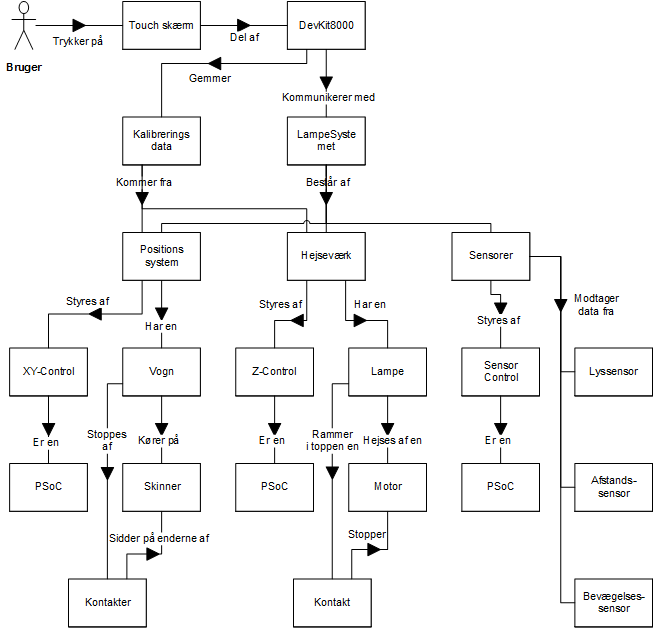
\includegraphics[width=\textwidth]{Filer/dmLAMP.png}
    \caption{Domænemodel L.A.M.P.}
    \label{fig:dmLAMP}
\end{figure}


\subsection{Blokdefinitionsdiagram}

På figur \ref{fig:bddLAMP} ses det overordnede BDD for systemet med de forskellige blokke det er blevet opdelt i. Et BDD er en overordnet beskrivelse af systemets blokke, med signaler, der går til og fra disse blokke der ud over fremgår det hvordan blokkene er forbundet med hinanden.

\begin{figure}[H] \centering
    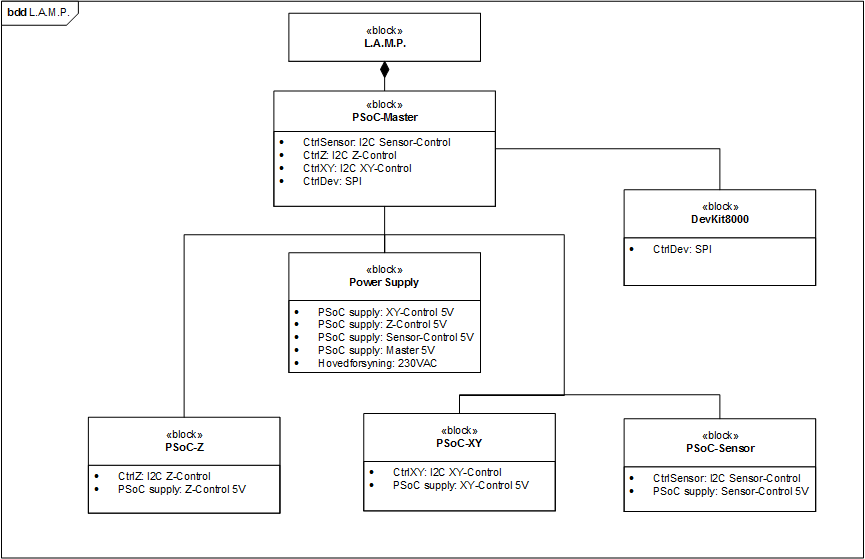
\includegraphics[width=\textwidth]{Filer/bddLAMPvers2.png}
    \caption{BDD L.A.M.P.}
    \label{fig:bddLAMP}
\end{figure}


\subsection{Intern blokdiagram}

På figur \ref{fig:ibdLAMP} ses IBD for det overordnede system. Her fremgår forbindelserne og signal navne mellem de forskellige blokke.

Som det fremgår af figur \ref{fig:ibdLAMP} er der 6 hovedblokke, som alle er en del af systemet L.A.M.P. Tre af disse blokke PSoC-XY, PSoC-Z og PSoC-Sensor består yderligere af dele som fremgå detaljeret af BDDer og IBDer i arkiteturdokumentet i bilag \footcite{documentation}.

\begin{figure}[H] \centering
    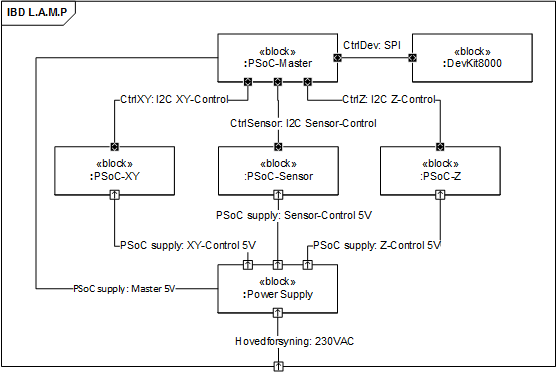
\includegraphics[width=\textwidth]{Filer/ibdLAMPvers3.png}
    \caption{IBD L.A.M.P.}
    \label{fig:ibdLAMP}
\end{figure}

\textbf{Beskrivelse af blokkene}

PSoC-Master: Denne blok står for al kommunikationen, den modtager kommandoer fra DevKit8000 via SPI kommunikation. Disse kommandoer sender den så via I2C kommunikation videre til den PSoC kommandoen omhandler.

PSoC-XY: Denne blok står for styringen af X og Y bevægelsen af systemet. Når den modtager en kommando fra PSoC-Masteren udføres den ønskede handling. 

PSoC-Z: Denne blok står for styringen af Z bevægelsen af systemet. Når den modtager en kommando fra PSoC-Masteren udføres den ønskede handling.

PSoC-Sensor: Denne blok styre og bearbejder data fra sensorene og RGB-dioden i systemet.

Power Supply: Som power supply til forsyning af systemet bruges en USB-hub som kan forsyne alle 4 PSoCs.

DevKit8000: Denne blok består af et bruger interface, det er her brugeren kan, via et touch display, sende ønskede kommandoer til systemet. 


% 4.4 Design
\section{Design}

\subsection{Hardware}

Systemet består af PSoC-Master som er forbundet til DevKit8000 med en 4-ledningers SPI-bus og forbundet til PSoC-XY, -Z og -Sensor med en 2-ledningers I2C-bus med eksterne pull-up modstande. Til test/debugning er der også brugt en UART forbindelse til at udlæse til Tera Term og en Nokia 5110 skærm til at aflæse indkommende og udgående kommuniaktion via SPI og I2C. På figur \ref{fig:psoc-master_topdesign} kan tilslutningerne for PSoC-Master ses.

% TopDesign PSoC-Master.
\begin{figure}[H] \centering
    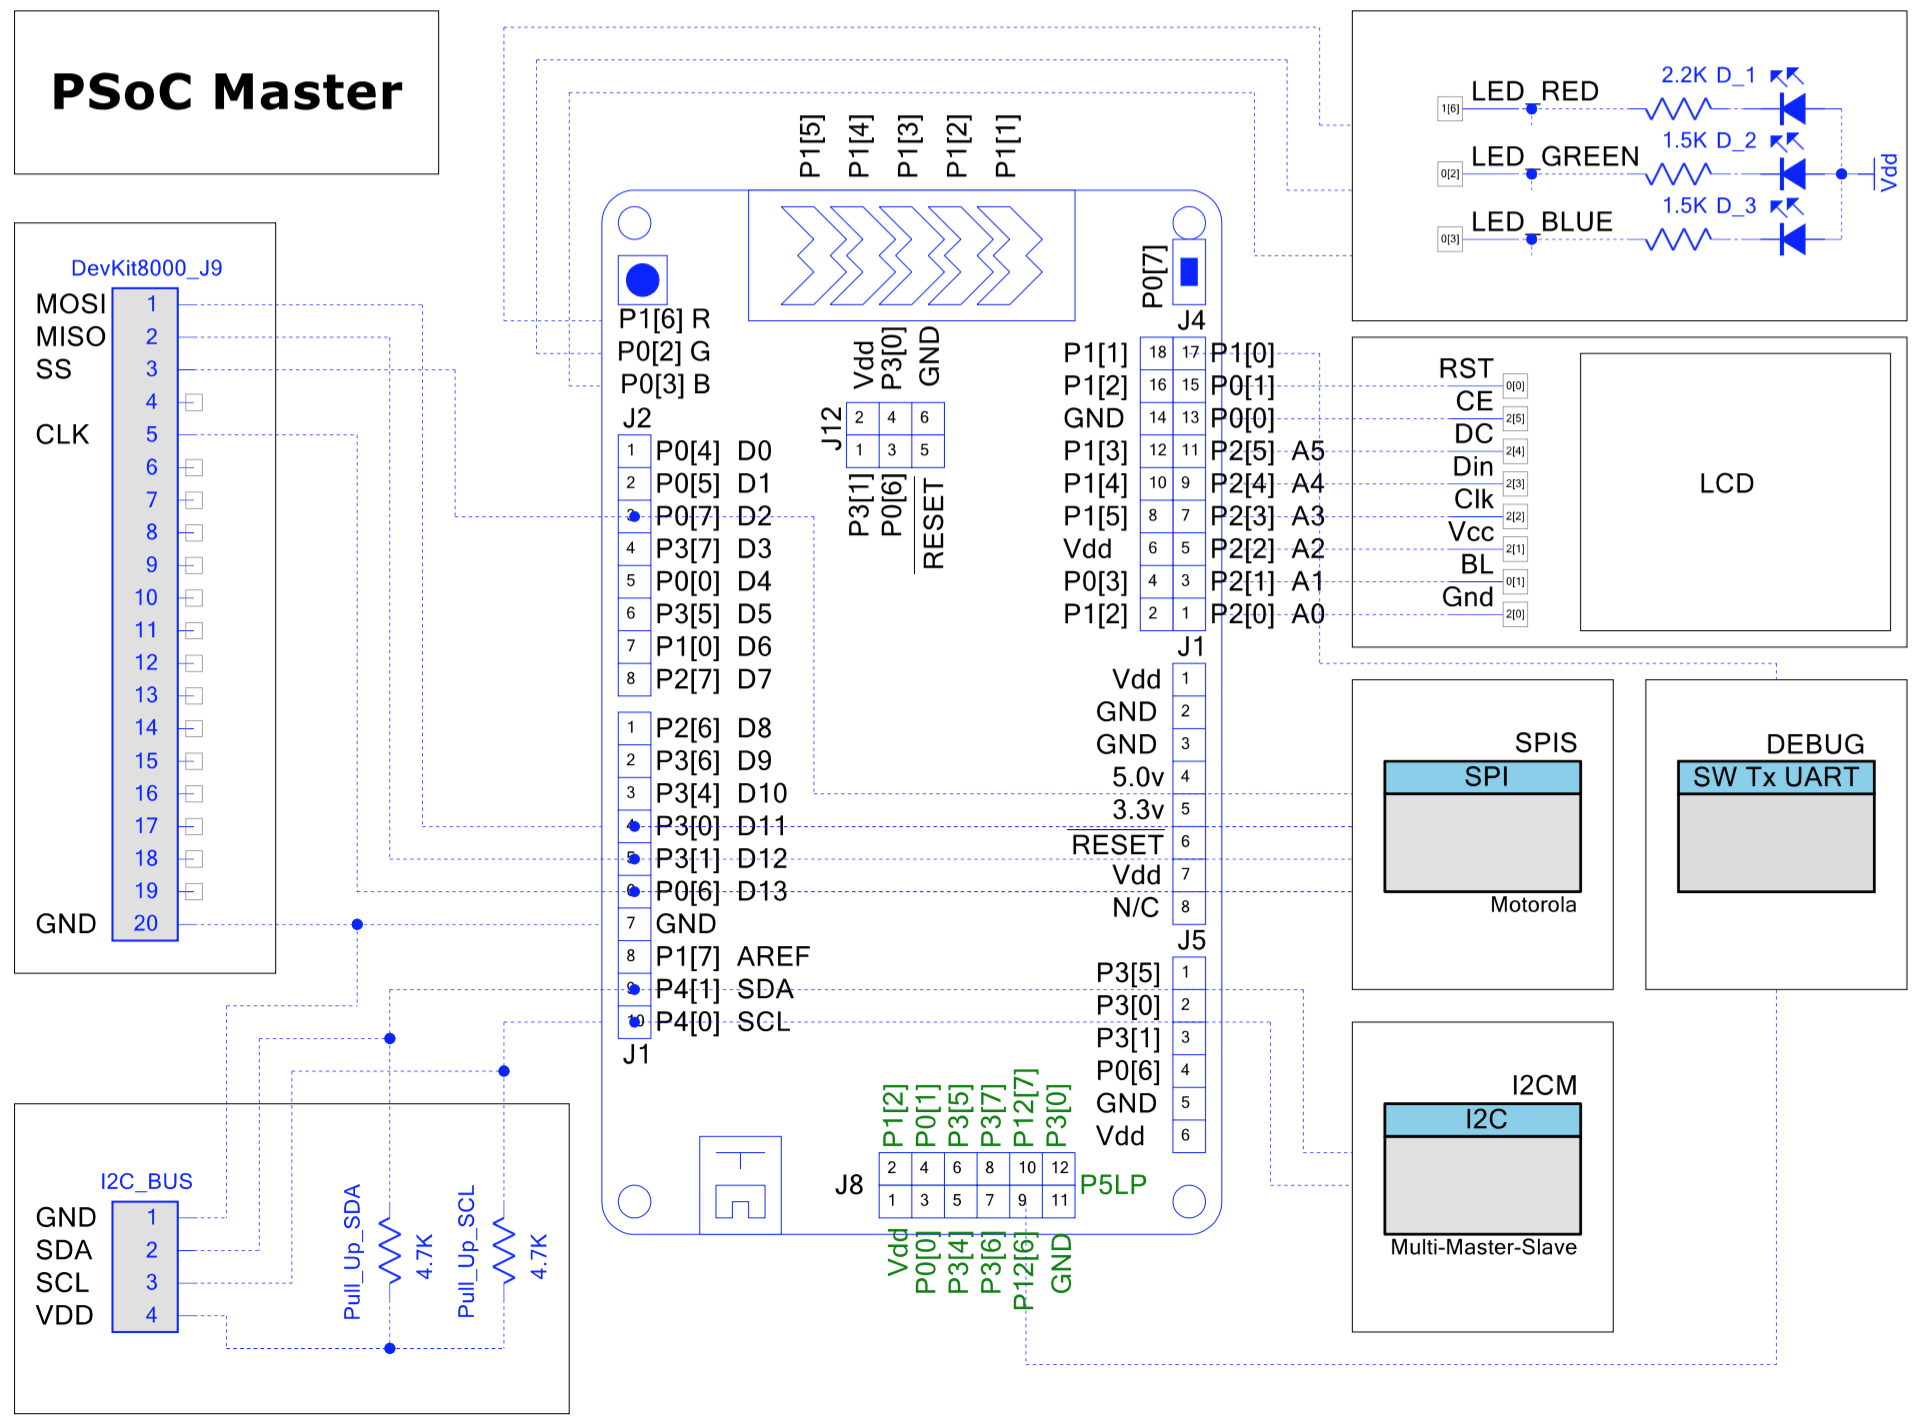
\includegraphics[width=\textwidth]{Filer/PSoC-Master_TopDesign.png}
    \caption{TopDesign PSoC-Master}
    \label{fig:psoc-master_topdesign}
\end{figure}

\subsubsection{Master-Blokken}
Systemet består af:
\begin{itemize}
	\item En PSoC\footcite{psoc}.
	\item Et Nokia 5110 display\footcite{nokia}.
\end{itemize}

Formålet med PSoC-Master er at den skal fungere som en "beskedcentral" mellem DevKit8000 og PSoC-XY, -Z og -Sensor.

Forbindelsen med DevKit8000\footcite{dk8000-addon} kører over SPI kommuniaktion, hvor DevKit8000 er SPI-master og PSoC-Master er SPI-slave.


\subsubsection{XY-Blokken}

Designet af XY blokken består af følgende 3 dele.

\begin{itemize}
    \item En PSoC\footcite{psoc}
    \item 4 stk. Stepper motor af typen (28BYJ-48) se databladet\footcite{28BYJ-48-5V} i bilag.
    \item 4 stk. Micro switches af typen (DM1-01P-30-3) se databladet\footcite{DM1-01P-30-3} i bilag.
\end{itemize}

For at kunne styre stepper motorerne er der implementeret en motorstyring. PSoC har 4 pins den sætter højt skiftevis, disse 4 pins giver et signal til motorstyringen, som alt efter hvilken pin der er aktiv, aktiveres en spole i motoren, som skifter polerne på en magnet. Dette sker ved at den tilslutter en stel forbindelse så der kan løbe en strøm i spolen. Magneten kan ved polskift få motoren til at bevæge sig. Ved at styre rækkefølgen af hvordan disse pins bliver sat høj kan man styre hvad vej motoren kører. Som ende stop på XY skinnerne er der blevet implementeret 4 switches/kontakter; 2 på X og 2 på Y. Kontakterne, ved aktivering, vil stoppe for den bevægelse der er i gang for at sikre systemets fortsatte drift. Yderligere bruges kontakterne ved kalibrering for at systemet kan registrere når lampen er nået til sine endepunkter på de pågældende skinner. 

Denne styring er stærkt inspireret af GFV\footcite{gfv}-øvelsen omkring stepmotorer.

\subsubsection{Z-Blokken}

Designet Z blokken består af følgende 3 dele.

\begin{itemize}
	\item En PSoC\footcite{psoc}.
	\item Én Stepper motor af typen (28BYJ-48) se databladet\footcite{28BYJ-48-5V} i bilag.
	\item Én Micro switch af typen (DM1-01P-30-3) se databladet\footcite{DM1-01P-30-3} i bilag.
\end{itemize}

Motoren til Z-aksen er styret på samme måde som motorerne for XY-delen.\footcite{documentation} Dvs. Motoren har 4 input pins + en 5 V VCC. Sættes de 4 input pins gentagende gange skiftevis til ground, i en bestemt rækkefølge, vil motoren kører rundt. Vælges den modsatte rækkefølge kører motoren baglæns.

Lampen hejses ned fra vognen med et fladt bånd. Køres lampen op vil den på et tidspunkt ramme en switch oppe under vognen. Til at signalere hvornår lampen er kørt langt nok ned, afhænger systemet af afstandssensoren, som sidder inde i lampen til at vurdere og markere hvornår en nedre grænse for Z-højden er nået.

\subsubsection{Sensor-Blokken}

Systemets sensorer er monteret direkte på bunden af vognen der kører på Y-aksen. Her er de forbundet til Z-vognprintet som giver den direkte forbindelse til PSoC-Sensor hvorfra de styres.

\subsection{Software}

\subsubsection{Kommunikation og databehandling}

Softwaren er fordelt ud på henholdsvis 1 Devkit8000 og 4 PSoC'er, med hver deres formål i produktet. Devkittet er brugerfladen, der viderebringer brugerinput og 1 af de 4 PSoC er beskedcentralen. Denne har til formål at distribuere input og output til de resterende PSoC'er baseret på de modtagene beskeder fra Devkittet. De resterende tre PSoC'er står for motorstyring i retning X, Y, Z samt styrer sensorerne.

Når et handlingsforløb påbegyndes, eventuelt ved tryk på devkittets touchskærm, vil inputtet blive tolket, sendt videre til beskedcentralen og derfra blive sendt videre til aktuelle PSoC-slave som har interesse i givne brugerinput. Givne PSoC-slave/r behandle dernæst disse data og produktets hardware vil skabe en respons. Denne procedure beskriver det generelle handlingsforløb fra Devkit8000 til hardware. 

Som eksempel på dette er der herunder opstillet en applikationsmodel, der beskriver kodeeksekveringen baseret på use-case 1 i dokumentationen. Denne use-case beskrive hvordan kalibrering af systemet bliver udført. For yderligere information om denne use-case, se dokumentationen sektion 2.3.1.


% {Applikationsmodel UC1
\begin{figure}[H] \centering
    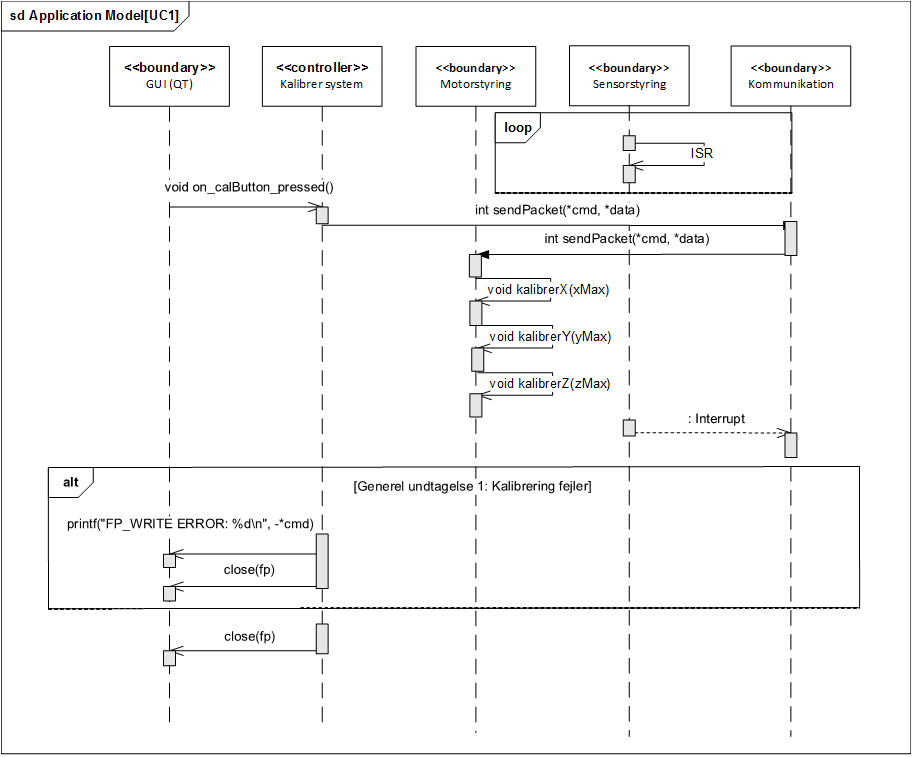
\includegraphics[width=\textwidth]{Filer/sdApplikationsmodelUC1.png}
    \caption{Applikationsmodel for UC1}
    \label{fig:sdUC1}
\end{figure}


\subsubsection{Devkit8000-Blokken}

Systemet består af:
\begin{itemize}
	\item Et Devkit8000\footcite{devkit}.
\end{itemize}

Devkit8000 har til formål at fungere som en fjernbetjening/styringsenhed til resten af systemet og være den del af systemet som brugeren aktivt skulle interagere med.

Devkit8000 indeholder en grafisk brugerflade (GUI) bestående af nogle grafiske elementer oprettet fra QT's designer. Disse elementer påvirkes live som et eventbaseret system, og er det brugeren kan se på Devkittets touchskærm. Når Devkittet påvirkes via touchskærmen bliver kode eksekveret i baggrunden afhængigt af brugerens handlinger. Handlingerne generere nogle signaler, der internt i koden udløser noget respons ved eksekvering af metoder. Hvad enten denne respons udelukkende foregår internt på Linux platformen eller sendes videre til resten af systemet vha. SPI-kommunikation er afhængigt af givne handling brugeren udfører. Alle handlinger bliver tracket i koden vha. signalerne med nogle tilhørende debugging-koder, der oplyser programmøren/debuggeren om, hvilken effekt givne handling havde for kodens udførsel og forløb. Brugeren kan som udgangspunkt kun se hvordan handlingerne påvirke det grafiske og er ubekendt med, hvad der sker i baggrunden.


Et eksempel på dette kunne være at et grafisk element, bestående af en slider, til styring af lampens position i x-aksen. Når denne sliders markørposition ændres vil en sliderværdi blive opdateret i koden, som en udvalgt metode (slot) kan benytte til enten at læse fra eller skrive til. Jævnfør dette eksempel nøjes, der med at blive læst fra slideren og det tilhørende slot (metode) er nu oplyst om at det grafiske element er blevet påvirket, og hvad dens værdier er på nuværende tidspunkt. Dette ville være et eksempel på beskedhåndtering internt i koden. Hvis brugeren vælger at denne værdi skal videreføres til resten af systemet/produktet, kan dette blive realiseret ved tryk på en Go-knap, der videresender x-sliderens positioneringsdata. Den satte dataværdi fra slideren bliver nu læst, behandlet og videresendt jævnfør SPI-API'en. Hvis kommunikationen sker fejlfrit vil PSoC Master videredistribuere data, og lampen vil bevæge sig. Hvis kommunikationen fejler vil fejlkoder blive returneret til Devkit8000 der kan ses vha. debugging gennem en terminal på en tilsluttet Linux-enhed.

For yderligere information henvises der til GUI-dokumentationen sektion 6.1.3 samt de tilhørende DoxyGen-filer\footcite{doxy-devkit}. 

\subsubsection{Master-Blokken}
PSoC-Masters software er delt op i følgende moduler

\begin{itemize}
    \item Data
    \item Handler
    \item I2C
    \item LED
    \item main
    \item Queue
    \item SPI
\end{itemize}

\textbf{Data}-structen indeholder værdier indhentet fra PSoC-XY, -Z og -Sensor.
Formålet er at DevKit8000 kan få hurtig adgang til disse. I tilfælde af at DevKit8000 skal bruge nogle data, vil denne først sende en "opdater værdier" kommando til PSoC-Master og derefter afvente et kort stykke tid inden den henter disse opdaterede værdier fra PSoC-Master. I mellemtiden går PSoC-Master ud til den relavante PSoC og henter de pågældende værdier og opdatere dem i data structen, så de er klar til at DevKit8000 kan hente dem.

I \textbf{handleren} modtages to parametere, hhv. kommando og værdi.
Herefter udføres der en funktion ud fra den modtagede kommando med den modtagede værdi.

Via \textbf{I2C} modulet sendes og hentes der pakker på I2C-bussen\footcite{scb}.
For at kunne gøre dette skal modulet have parametrene for modtageradressen, kommandoen og værdien der skal sendes med.

\textbf{LED} kan tænde/slukke PSoC-Masters red-, green- og blue-LED. Dette bruges i forbindelse med kommunikationen til at angive aktivitet og om pakker er blevet afsendt eller fejlet.

Hovedprogrammet \textbf{main} intialiserer modulerne og køre derefter loop hvor der bliver kontrolleret om der er nogle actions i køen der skal håndteres af handleren.

\textbf{Queue} håndterer køen der er bygget op af en FIFO queue der bruger en linked list til at håndterer elementer med.

Modulet \textbf{SPI} modtager og håndter data pakker fra DevKit8000 via SPI-busset\footcite{scb} og opdatere data i SPI bufferen til aflæsning fra DevKit8000.

Når DevKit8000 sætter SS lav starter en ISR routine på PSoC-Master. DevKit8000 sender så via SPI-protokolen en 16-bit pakke til PSoC-Master og sætter herefter SS høj igen, for at afslutte.
PSoC-Master bearbejder herefter det modtagede 16-bit data og deler det op i to stykker; en kommando og en værdi.
Kommandoen og værdien bliver pakket ind i en struct og sat ind i en FIFO\footcite{fifo} kø.
I hovedprogrammet på PSoC-Master bliver der løbende kontroleret om der er data i køen der skal håndteres, når dette er tilfældet trækker den dataen ud af køen og sender det til handleren i form af kommando og værdi. I handleren bliver der kigget på hvilken kommando der er modtaget og ud fra kommandolisten bliver der foretaget den handling som vedrører kommandoen. 

Hvis kommandoen f.eks er at sætte en X position, vil handleren kalde I2C-setfunktion med paremeterene for: modtagers I2C-adresse, kommando og værdi. I2C funktionen pakker den modtagede kommando og værdi i en buffer til I2C afsending. I bufferen er der også blevet tilføjet en SOP\footnote{Start of packet} og en EOP\footnote{End of packet} som bliver sendt med som den første og sidste byte i kommunikationen. Disse bytes bliver brugt af modtageren til at kontrollere at det modtagede data er validt.

Når kommandoen er afsendt og handleren er færdig med opgaven, vil programmet gå tilbage til hovedprogrammet, hvor det fjerner dataen i køen. Derefter kigger det i køen om der er mere data der skal behandles.


\subsubsection{XY-Blokken}

Dele af PSoC-XY softwaren er opbygget med samme moduler som på PSoC-Master, herunder modulerne data, handler, LED, main og queue.

Der er ydermere tilføjet/ændret disse moduler
\begin{itemize}
    \item Data
    \item I2C
    \item LED
    \item XY
\end{itemize}

\textbf{Data} modulet håndterer værdierne for XY såsom den nuværende position, max position, er enheden kalibreret og hvilken vej kører enheden.

\textbf{I2C} modtager data pakker fra PSoC-Master og bearbejder dem til en action som indsættes i køen til håndtering i hovedprogrammet.

\textbf{LED} kan tænde eller slukke PSoC-XYs LEDs. Dette bruges til at indikerer om PSoC-XY'en er i gang med at udføre en opgave, kalibere eller modtager et interrupt.

Modulet \textbf{XY} håndterer funktionaliteten til hardwaren og bliver kaldt fra handleren med en specifik opgave. Ydermere håndterer den de interrupts der kan forkomme fra hardwaren. 

\textbf{Strømløs tilstand} kan forekomme ved strømafbrydelser eller lignende. PSoC-XY håndtere dette ved at positionere sig i 0/0 på X- og Y-aksen når strømmen atter er genoprettet. Dette gør den ved at aktivere motorerne i retningen mod nulpunktet på akserne, og stopper ved aktivering af interrupt. 

\subsubsection{Z-Blokken}

PSoC-Zs software er stort set identisk med PSoC-XY, dog er XY-modulet udskiftet med et Z-modul som er tilpasset hardwaren på PSoC-Z.

\textbf{Strømløs tilstand} kan forekomme ved strømafbrydelser eller lignende. PSoC-Z håndtere dette ved at køre lampen op til der registreres et interrupt på Z-switchen.

\subsubsection{Sensor-Blokken}


\begin{figure}[H] \centering
    \includegraphics[width=0.8\textwidth]{Filer/PSoC-Sensor-TopDesign.PNG}
    \caption{TopDesign PSoC-Sensor \footcite{dk8000-addon}}
    \label{fig:Sensor-top}
\end{figure}

Som det fremgår af figur \ref{fig:Sensor-top} består PSoC-Sensor af 7 blokke på TopDesign niveau, hvoraf de mest interessante er:

\begin{itemize}
	\item Afstandssensor
	\item LED PWM
	\item Main loop metronom
	\item Debug
\end{itemize}

For at aflæse afstandssensoren skal der kunne måles hvor længe en pin bliver holdt høj, med en præcision på et par mikrosekunder (1 cm svare til 58 us). Derfor er der sat en timer op med en 1 MHz clock, der starter med at tælle på rising edge af det signal der skal måles, og derefter stopper, gemmer tællerværdien og starter en interrupt på falling edge.

Denne blok har desuden tre ekstra pins: DistTrigger, DistReset, og DistInterruptPin. DistTrigger bruges til at starte målingen - sensoren skal have en 10 us puls som input før den starter. DistReset bruges til at resette timeren mellem målingerne, da den ellers blot fortsætter med at tælle derfra hvor den kom til. Til sidst bruges DistInterruptPin til at sende et signal direkte til PSoC-Z når afstandssensoren måler at vi er kommet for tæt på en underliggende forhindring.

De tre LEDs styres med PWM, og hver farve (rød, grøn, blå) har sit eget PWM modul. De deler dog alle tre clock med afstandssensor-timeren. Dette er valgt fordi PSoC4 maksimalt understøtter fire brugerdefinerede clocks, så når forskellige komponenter kan sættes til at virke med samme clock-frekvens, er der ingen grund til at bruge flere resourcer end nødvendigt.

Metronom blokken indeholder en timer der er sat til at lave et interrupt hvert halve sekund. De interrupts bliver så brugt i hovedprogrammet til at aktiverer sensoraflæsninger og andre periodiske events. Denne timer har sin egen clock (200 Hz), da det gjorde designet nemmere og lod os holde timeren på 8 bits, hvilket sparer andre resourcer i PSoC'en.

Den sidste blok er Debug. Den indeholder et UART modul, men da de to I2C moduler optager alle de dedikerede hardware kommunikationsblokke, så bliver der her brugt et software modul der kun understøtter transmit.

Strømløs tilstand håndteres I PSoC-Sensor ved at systemet ved opstart initializerers med fornuftige opstartsværdier. F.eks. starter den med lyset slukket og en afstandssensor alarm grænse på 10 cm.


% 4.5 Implementering
\section{Implementering}

\subsection{Hardware}

Hardwaren på produktet er bygget fra bunden. Rammen som prototypen står på er taget fra et gammel metal-stel, men udover dette er resten konstrueret af gruppens medlemmer. Skinnerne er skåret i kabelføringsbakker og det samme er vognene. Alt er skruet og samlet af gruppen selv. 

Systemets PSoC'er er samlet under ét fordelingsprint. Dette print samler dataene fra PSoC-XY, -Z, og -Sensor og sender dem videre ud til enten motorerne eller sensorerne. 

% Fordelingsprint
\subsubsection{Fordelingsprint}
\begin{figure}[H] \centering
    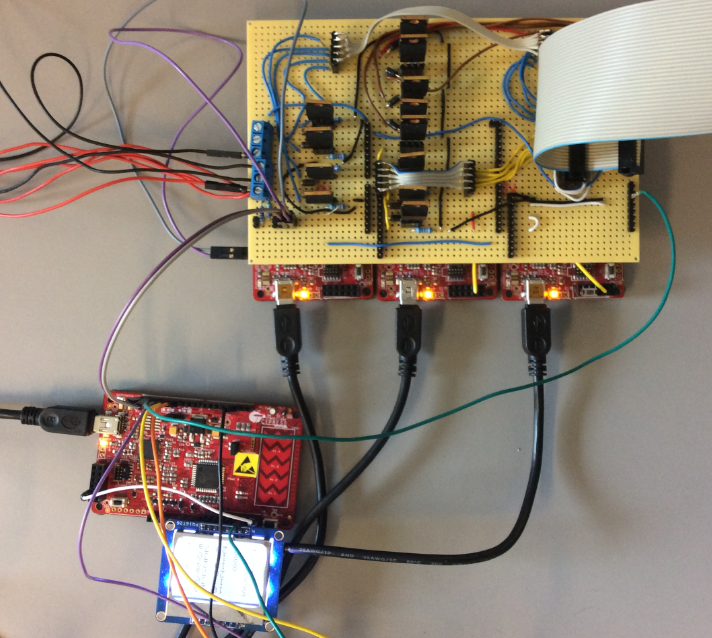
\includegraphics[width=0.6\textwidth]{Filer/FordelingsPrint.PNG}
    \caption{Fordelingsprint}
    \label{fig:Fordelingsprint}
\end{figure}

På figur \ref{fig:Fordelingsprint} ses fordelingsprintet. Dette print er bygget med pins så det kan sættes på XY-, Z- og Sensor PSoCs og dermed slippe for alt for mange ledninger. Printet indeholder hardwaren til I2C-kommunikation mellem PSoC-Master og de resterende PSoCs samt tre motorstyringer til henholdsvis X, Y og Z-motorerne. Derud over er printet forbundet med motorene, sensorerne og LED'erne\footcite{L-154A4} via. et 34 leder kabel.
For printlayout og diagram, Se dokumentationsrapporten\footcite{documentation}.

% X Moter Montering
\subsubsection{X Motor Montering}
\begin{figure}[H] \centering
    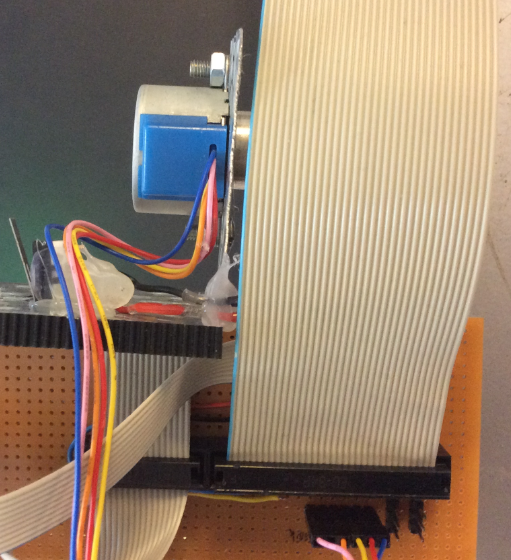
\includegraphics[width=0.5\textwidth]{Filer/XMotorMont.PNG}
    \caption{X Motor Montering}
    \label{fig:XMotorMont}
\end{figure}

På figur \ref{fig:XMotorMont} ses tilslutningen af 34 leder kablet fra fordelerprintet samt monteringen af den ene af X-motorerne. Fra denne tilslutning bliver signaler, spændinger og kommunikation fordelt ud til deres respektive enheder. For printlayout og diagram, Se dokumentationsrapporten\footcite{documentation}.

% Z Motor Montering
\subsubsection{Z Motor Montering}
\begin{figure}[H] \centering
    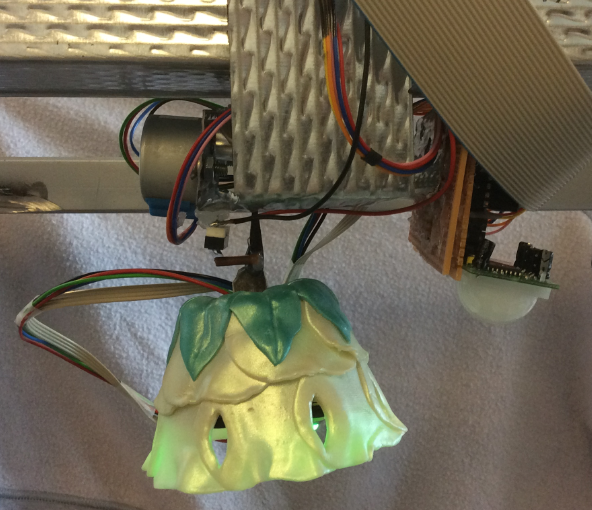
\includegraphics[width=0.6\textwidth]{Filer/ZMotorMont.PNG}
    \caption{Z Motor Montering}
    \label{fig:ZMotorMont}
\end{figure}

På figur \ref{fig:ZMotorMont} ses bunden af Z-vognen. Det er her Z-motoren, lampen med RGB dioder\footcite{L-154A4} samt systemets sensorer er monteret. For printlayout og diagram, Se dokumentationsrapporten\footcite{documentation}.

\subsection{Software}

I projektet er der brugt både C og C++. Alt PSoC software er skrevet i C da det er det sprog PSoC Creator understøtter. Desuden er SPI driveren til DevKit8000 skrevet i C, fordi den er skrevet som et Linux-kernemodul og det kræver igen C. Sidst men ikke mindst er GUI'en på DevKit8000 skrevet i C++ med brug af QT biblioteket.

\subsubsection{Devkit8000}

På Devkit8000 er de mest interessante moduler:

\begin{itemize}
	\item position
	\item light
	\item settings
\end{itemize}

\textbf{Position} er den kodesektion der beskriver hvordan lampen skal bevæge sig på de tre akser. Kodesektionen håndterer videreførelsen af de beskeder som brugeren opretter gennem position-fane. Det særligt interessante består i den grafiske repræsentation, bestående af et koordinatsystem, skal stemme overens med den reelle positionering af produktet. Således kan brugeren virtuelt blive repræsenteret for, hvordan systemet vil blive påvirket såfremt brugeren vælger at realisere disse ved at videresende vha. SPI.

\textbf{Light} er den kodesektion der beskriver lysstyringen for lampens RGB-LED'er\footcite{L-154A4}. På samme måde som ved position, viderekommunikeres brugeraktionen på de grafiske elementer til systemet, såfremt dette vælges af brugeren, og genererer desuden en virtuel repræsentation. I dette tilfælde repræsenteres værdierne med en farve palette med den blandede farve bestående af de tre værdier. Særligt interessant er det her, at præsentere for brugeren hvordan interaktionen påvirker systemet forinden det bliver viderebragt og påvirker lampens lys.

\textbf{Settings} kodesektionen står for den generelle sensorkontrol. Man kan her både ved bevægelsessensoren og lumensensoren betragte Devkit8000 som en afbryder, da disse kun kan ændres til to tilstande; tændt og slukket. Den sidste sensor der påvirkes i denne sektion er afstandssensoren, der altid er aktiv. Denne kan påvirkes med hensyn til hvilken afstand den skal alarmere resten af systemet. Brugeren får gennem denne sektion frirum til at til- eller fravælge sensorfunktionalitet og indstille på dem.

\subsubsection{Master}

Særligt interresant i softwaren på PSoC-Master er \verb+isr_spi_rx()+ og \verb+i2c_tx()+ funktionerne, da de er bærende element i hele funktionaliteten.

\subsubsection{SPI}

%TC:ignore
\lstinputlisting[language=C,caption={isr\_spi\_rx()},label={listing:isrspirx}]{Filer/isr_spi_rx.c}
%TC:endignore

\verb+isr_spi_rx()+ Listing \ref{listing:isrspirx} er en \verb+Interrupt service routine+ som afvikles ved modtagelse af data via SPI-busset. Det modtagede data bliver læst ind på en buffer fra SPI komponenten, hvorefter det deles op i en kommando og en værdi. Alt efter hvilken kommando der er modtaget fortages en defineret handling. 


\subsubsection{I2C}

%TC:ignore
\lstinputlisting[language=C,caption={i2c\_tx()},label={listning:i2ctx}]{Filer/i2c_tx.c}
%TC:endignore

\verb+i2c_tx()+ Listing \ref{listning:i2ctx} funktionen bruges til afsendelse af datapakker på I2C-bussen. Når funktionen kaldes sendes der en addresse, kommando og værdi. Kommandoen og værdien sættes ind i en buffer til afsendelse. I bufferen er der også tilføjet en \verb+Start of packet (SOP)+ byte og en \verb+End of packet (EOP)+ byte, disse sættes ind hhv først og sidst i bufferen og bruges af modtageren til at kontrollere om den fulde pakke er modtaget.
Herefter kaldes en \verb+I2CM_I2CMasterWriteBuf()+ med modtager adressen, bufferen til afsendelse, buffer størelsen og mode for afsenelse, som er komplet afsendelse her. Derefter afventer funktionen at pakken er blevet korrekt afsendt og derefter nustiller I2C komponemtets status.


\subsubsection{XY I2C}

%TC:ignore
\lstinputlisting[language=C,caption={I2CS\_I2C\_ISR\_ExitCallback()},label={listning:i2csi2cisrexitcallback}]{Filer/I2CS_I2C_ISR_ExitCallback.c}
%TC:endignore

\verb+I2CS_I2C_ISR_ExitCallback()+ Listing \ref{listning:i2csi2cisrexitcallback} er en \verb+Interrupt service rotine+ som automatisk kaldes efter der er modtaget en datapakke over I2C-bussen.
Det modtagede data lagres ind i en struct og alt efter hvilken kommando der er modtaget fortages en defineret handling. Efterfølgende nulstilles SPI komponentens status.

\subsubsection{X-, Y- og Z-Styringskode}

Styringen af systemets motorer foregår via PSoC-XY og PSoC-Z. Disse PSoC'ere har deres eget program, som styrer hvilken handling de skal tage. De modtager gennem I2C to variable; en kommando og en værdi. Disse variable bruger de til at identificere deres handlinger og igangsætte de definerede funktioner.  


Funktionerne er som følger: \newline
\verb+SetXPos(uint XVal);+  \newline
\verb+SetYPos(uint Yval)+   \newline
\verb+SetZPos(uint Zval)+   \newline
\verb+StepXForwards();+     \newline
\verb+StepXBackwards();+    \newline
\verb+StepYForwards();+     \newline
\verb+StepYBackwards();+    \newline
\verb+StepZForwards();+     \newline
\verb+StepZBackwards();+    \newline
\verb+CalibrateX();+        \newline
\verb+CalibrateY();+        \newline
\verb+CalibrateZ();+        \newline
\verb+CY_ISR(isr_X);+	    \newline
\verb+CY_ISR(isr_Y);+	    \newline
\verb+CY_ISR(isr_Z);+	    \newline



\textbf{StepForwards / StepBackwards}\newline 
Når en position bliver valgt på Devkit8000 er det PSoC-XY og PSoC-Z der skal sørge for at positionere lampen til den valgt placering. Kommando-variablen bruger den til at definere hvilken motor der skal aktiveres, og værdi-variablen bruger den til at finde ud af hvor den skal kører motoren hen. 

Hvis motoren befinder sig i position 100 på X-aksen, gemt i variablen xPos, og kommandoen for aktivering af X-motor, SetXPos(), bliver kaldt, samt værdien der bliver modtaget er 150, vil PSoC-XY trække sin nuværende position fra den modtagede værdi. 150 minus 100 giver 50. da 50 er et positivt tal, vil StepXForwards() blive kaldt med værdien 50, altså; StepXForwards(50);
Hvis den sendte værdi var 50, ville resultatet give -50. Her vil StepXBackwards() blive kaldt med værdien 50, altså; StepXBackwards(50);
Dette er gældende for motorstyringen på alle tre akser. 

\textbf{Calibrate();}\newline 
Dette funktionskald aktiverer X-motorerne i den ene retning. Når retningens grænse er nået, vil en fysisk afbryder blive aktiveret og herved levere besked gennem CY\textunderscore{}ISR(isr\textunderscore{}) til PSoC-XY om at den nedre grænse er nået. Herefter vil X-motorerne køre i den anden retning til de rammer den øvre grænse hvor endnu en afbryder bliver aktiveret. \newline 
De steps motoren tager imellem den nedre og øvre grænse bliver gemt i en værdi kaldet xMax. Motorens nuværende position ved den øvre grænse gemmes i en variabel kaldet xPos som bliver sat til 0. 
\newline 
Når xMax og xPos er sat, aktiveres Y-motorerne i den ene retning. Når retningens grænse er nået, vil en fysisk afbryder blive aktiveret og herved leverer besked til PSoC-XY om at den nedre grænse er nået. Herefter vil Y-motorerne køre i den anden retning til de rammer den øvre grænse hvor endnu en afbryder bliver aktiveret. 
\newline 
Her bliver antal steps Y-motorerne har kørt gemt i en variabel kaldet yMax, og motorens nuværende position bliver gemt i en variabel kaldet yPos som sættes til 0. 
\newline
Fremgangsmåden som PSoC-Z bruger til at kalibrere sine værdier med, er meget lig den PSoC-XY benytter. Den kører lampen ned med SetZForwards() til den får et interrupt af afstandssensoren. Ved dette interrupt er den nedre grænse nået, og PSoC-Z vender nu motorens retning, og tæller antal steps op til næste interrupt. Den gemmer antal steps mellem de to interrupts i zMax, stopper ved øverste interrupt og sætter sin position i zPos til 0.
Hermed er skinnernes længde målt ud, rummets dybte målt ud, lampens position er sat og systemet er nu kalibreret.

\textbf{CY\textunderscore{}ISR(isr\textunderscore{})}\newline 
Ved skinnernes ydre grænser og ved lampens topposition sidder der Micro switches monteret. Ved aktivering slutter disse en kreds der levere 5V på den definerede pin på PSoC'en. når denne sættes igang, aktiveres Interrupt Service Rutinen. Denne stopper motoren på den pågældende akse, og igangsætter motoren den modsatte vej med 50 steps. At motorerne kører 50 steps tilbage er vigtigt for ikke at hvile på kontakten og have en konstant aktiveret interrupt der forhindre programmet i at gøre andet. 



% Sensor
\subsubsection{Sensor}

I PSoC-Sensor er de mest interessante moduler:

\begin{itemize}
	\item handler
	\item LumenSensor
	\item main
\end{itemize}

Modulet \textbf{handler} håndterer PSoC-Sensors opførsel når den modtager I2C kommandoer fra PSoC-Master. Basalt set én stor switch, med en case for hver kommando PSoC-Sensor kan modtage og håndtere.

\textbf{LumenSensor} er det software modul der håndterer I2C kommunikationen med lyssensoren. Dette har fået sit eget modul da en enkelt aflæsning af sensoren består af at skrive en byte til sensoren, læse to bytes fra sensoren, og derefter skrive en og læse to bytes igen.

 \textbf{main} indeholder den overordnede kontrolstruktur i PSoC-Sensor, der bestemmer hvornår alt andet skal køres. Som beskrevet ovenfor i TopDesign, så er hjertet Metronom timeren der giver et taktslag hver halve sekund. For hvert taktslag bliver en række tællere talt op og tjekket for overløb. Hver tæller der løber over bliver nulstillet og hæver et flag. De flag bliver tjekket i hoved-løkken og den tilhørende kode bliver udført.

Alt i alt gør denne opbygning at der kan defineres periodiske events med individuelle perioder (med en opløsning på 0.5 sekunder). Det giver den fordel at vi kan have en hoved-løkke der kører hele tiden, uden at blive standset af delay kommandoer, hvilket giver muligheden for et mere responsiv og jævnt kørende program. Men samtidig undgår vi at overbelaste sensorene ved at aktiverer dem alt for ofte.

Til sidst bør det nævnes at systemet bruger et \textbf{lux} modul som vi ikke har skrevet selv. Den er kopieret fra lumen sensorens datablad\footcite{TSL2561}.


% 4.6 Test
\section{Test}

For at sikre et stabilt og funktionelt produkt er der blevet gennemført tests af systemet. Systemet er løbende, gennem hele udviklings processen, blevet modultestet og integrationstestet, det vil sige at når der løbende er blevet implementeret dele på projektet er de blevet testet til den ønskede funktionalitet og præcision er opnået. Som afslutningstest af hele systemet, blev den tilhørende udspecificerede accepttest gennemført. Se accepttest under kravspecifikation i bilags sektionen. 

\subsubsection{Test forløb}
Gennem hele forløbet er der blevet testet for at sikre et acceptabelt produkt. Testene er løbene blevet gennemført i et samarbejde, mellem gruppens medlemmer for at kunne få alle modulerne til at kommunikere mellem hinanden. Produktet blev bygget systematisk op, så hele prototypens konstruktion blev bygget først samt. implementeringen af X Y modulet. Efter X og Y positioneringen og kommunikationen til PSoC-Master og DevKit var testet og oppe og køre, blev samme procedure udført for Z modulet og Sensor modulet. Ved test af sensor modul skulle de forskellige sensorer også testes og justeres, b.la. skulle bevægelsessensoren(P.I.R) testes og justeres så den var tilpasset prototypens størrelse. Dette samme gjorde sig gældende for afstandssensoren, for at sikre en sikker bevægelses zone for lampens hejse funktion.

Til test af XY og Z positionering blev Capsense slider-funktionen implementeret på de to PSoCs. Dette gjorde det muligt at manuelt teste kørslen af motorene i forskellige retninger samt at teste hele prototypens konstruktion. På denne måde kunne det observeres på hvad der fungerede og hvad der ikke gjorde og få ombygget og rekonstrueret eventuelt dårlige konstruktioner.

Til test af kommunikationen mellem Devkit8000 og modulerne, samt at kunne have et overblik over kommandoer i kø, blev der implementeret et Nokia5110 display på PSoc-Masteren. Dette display gjorde det muligt at se hvis kommunikationen fejlede mellem Devkit8000 og PSoC-Masteren og visse køens indhold.

Til test af hele software delen er der blevet brugt Tera Term, som gjorde det muligt at visse hvor eventuelle fejl var opstået i programmet. %Her skal indsættes nogle referencer.

\subsubsection{Accepttest}
Accepttesten er blevet udført efter modultest og integrationstest. Accepttesten er opbygget så den kan udføres af en hvilken som helst person. Gennemførelsen af accepttesten, dokumenteret i kravspecifikationen under bilag, er blevet udført af gruppen. Dette blev gjort ved at køre testen igennem punkt for punkt og udføre de gennemførte introduktioner der er beskrevet og der efter noterer resultatet i de her til tilhørende rubrikker. Testen er bygget op så denne gennemgår samtlige usecases der er, det vil sige at alle tænkelige funktioner i systemet bliver testet.

Til fejlfinding eller andet vil accepttesten til hver en tid kunne gengennemføres. Hvis dette ønskes henvises der til kravspecifikationen under bilag.   


% 6. Resultater
% 5. Resultater
\chapter{Resultater}

\section{Accepttestresultater: }
De 5 Accepttests er gennemført og resultaterne for disse er opsummeret i den følgende tabel.

\begin{center} \centering
    \begin{longtable}{|p{0,5cm}|p{3,7cm}|p{3,7cm}|p{2,3cm}|p{2,3cm}|}
    \hline
        \multicolumn{5}{|l|}{\textbf{Accepttestresultater }} \\ \hline
        \multicolumn{1}{|c|}{} &
        \textbf{Test} &
        \textbf{Forventet \newline Resultat} &
        \textbf{Resultat} &
        \textbf{Godkendt\slash \newline Kommentar} \\ \hline 
        \endfirsthead

        \multicolumn{5}{l}{...fortsat fra forrige side} \\ \hline 
        \multicolumn{5}{|l|}{\textbf{Accepttestresultater }} \\ \hline
        \multicolumn{1}{|c|}{} &
        \textbf{Test} &
        \textbf{Forventet \newline Resultat} &
        \textbf{Resultat} &
        \textbf{Godkendt\slash \newline Kommentar} \\ \hline 
        \endhead

        \multicolumn{5}{r}{fortsættes på næste side...} \\
        \endfoot
        \endlastfoot
        
        \textbf{1} 
            & \textbf{Kalibrer system}\newline
Brugeren kalibrerer systemet for X-, Y- og Z-aksen
            & Lampen bevæger sig ud i de tre aksers maksværdier og gemmer data.
            & Lampen nåede alle maksværdierne som fejlfrit blev returneret og gemt.
            & Godkendt.
        \\ \hline
        \textbf{2} 
            & \textbf{Tænd/sluk lys}\newline
Brugeren kan tænde og slukke lyset med On-/Off-knapperne på touchskærmen.
            & Lyset forventes tændt med de sidst sendte farveindstillinger ved tryk på On og slukket helt ved tryk på Off
            & Lyset tændte med den valgte farve og slukkede som forventet. 	
            & Godkendt.
        \\ \hline
        \textbf{3} 
            & \textbf{Registrer bevægelse}\newline
Brugeren tænder lyset med sidst sendte farveværdi ved hjælp af bevægelsessensoren ved at skabe bevægelse inden for sensorens rækkevidde.
            & Lyset forventes at tænde med sidst sendte farveværdier når bevægelsessensoren registrerer bevægelse.
            & Lyset tændte med korrekt farve, når bevægelse blev registreret.	
            & Godkendt.
        \\ \hline
        \textbf{4} 
            & \textbf{Juster lysets farve}\newline
Brugeren ændrer lysets farve ved at flytte de tre farvesliders og sender værdierne ved tryk på Go-knappen. 
            & Lampen forventes tændt med samme farveværdi som fremvist på touchskærmens farvepalette.
            & Farven fra lampen stemte overens med den på touchskærmen fremviste på farvepalette.	
            & Godkendt.
        \\ \hline
        \textbf{5} 
            & \textbf{Instilling af lampens placering}\newline
Brugeren sætter en valgt position for X-,Y- og Z-aksen og trykker på Go-knappen.
            & Lampen bevæger sig hen til den korresponderende placering der stemmer overens de sendte sliderværdier.
            & Lampen bevægede sig til den valgte placering i alle tre akser.	
            & Godkendt.
        \\ \hline
	\end{longtable}
	\label{Accepttest}
\end{center}


% 7. Diskussion af resultater
% 7. Diskussion af resultater
\chapter{Diskussion af resultater}
Ud fra de gennemførte accepttests kan det konstateres at prototypen på L.A.M.P. er en success.
Lampen kan bevæge sig fejlfrit på X- og Y-aksen. på Z-aksen er der en tendens til at lampen ikke altid hejses fejlfrit, da der sidder en lille klump lim oppe under motoren som til tider kan løfte båndet op fra hjulet som trækker båndet rundt. Det kan i værste tilfælde få båndet til at glide af så lampen falder et par cm og snoren bliver viklet.

Hvad sensorerne angår, virker afstandssensoren og bevægelsessensoren i systemet. Afstandssensoren kan aktiveres og deaktiveres samt finjusteres via GUI'en.

Bevægelsessensoren kan også aktiveres og deaktiveres via GUI'en, og er meget effektiv til at opfange bevægelse. Selv når man går rundt om prototypen kan bevægelsessensoren bemærke det.

Lyssensoren fungerer teknisk set i opsætningen. Dvs. den kan detektere et samlet lysniveau og systemet kan tolke dets målinger. Desværre ligger lysmålingerne der kommer fra diodernes lys, så lave og ens, at der ikke kan tolkes noget ud fra om dioderne tilføjer noget markant til den samlede lysstyrke.

Lysdioderne virker helt som de skal; De kan tændes og slukkes, og deres farve kan ændres efter deres indstilling på touchskærmen. Selve lyset fra dioderne er dog ikke stærkt nok i forhold til at de skulle fungere som lyskilder til et lokale.

% 8. Fremtidigt arbejde
% 8. Fremtidigt arbejde
\chapter{Fremtidigt arbejde}

Efter at have arbejdet med produktet og udviklet på produktet løbende, er det nået til det stadie der opfylder de af gruppen fastsatte krav. Men selvom produktet er færdigt, er der stadig udvidelser eller direkte tilføjelser der kan give kunden mere værdi.

\textbf{Mangler for projektets færdiggørelse:}
Under feltet afgrænsning ”TODO:HENVISNING” er det beskrevet at produktet ikke har fået implementeret sin lumensensor. Dette ville være anderledes, var der givet en større tidsramme. Yderligere var farvetemperatursensoren også en overskuelig komponent at få implementeret. Hvis der blev givet mere tid til produktet ville tiden også blive brugt på at arbejde med de sidste små bugs og glitches i koden. Yderligere ville den fysiske fremstilling af produktet også nyde godt af at få lidt opmærksomhed. 

\textbf{Fremtidige udvidelser eller udviklinger:}
Som beskrevet under afgrænsning ”TODO:HENVISNING” er det muligt at udvide produktet med flere hardwarekomponenter der giver flere features. Trådløs betjening er meget oppe i tiden, og er ofte forventet ved køb af nye husholdningsinstallationer, hvorfor det ville være et stort plus for produktet at have netop denne feature. Ligeledes ville en tilføjelse af et gsm-modul også give kunden mulighed for at styre produktet trådløst. Yderligere ville produktet kunne udvides til at kunne styres med en app til smartphones.

Selve rammen for produktet har mange anvendelsesmuligheder. Det behøver ikke nødvendigvis at være til at flytte belysningen i et rum. I stedet for en lampe, kunne der påmonteres en krog med en straingauge og man ville have en værkstedskran der ville kunne måle om det emne det skulle løfte ville være for tungt til rammens kapacitet. I stedet for en krog, ville man kunne montere en elektromagnet og man ville kunne flytte kasser med metallåg på et lager. Da produktet har mulighed for at gemme positioner, ville den også kunne gemme hvilke positioner den stiller de forskellige kasser på, og dermed ville man have et særligt lagersystem.

Som en omdannelse af produktet ville det være muligt at erstatte vores lampeledning med en gevindstang og påmontere et printerhoved på enden af denne gevindstang. Derved ville man ændre produktet fra en lampe til en 3D-printer. Dette er dog mere en ændring end det er en udvidelse eller en udvikling af produktet.    


% 9. Konklusion
% 4. Konklusion (samlet)
\chapter{Konklusion (samlet)}

Som gruppe er vi kommet godt igennem udviklingsprocessen og har fået skabt et godt produkt. Det er lykkes os at implementere vores målsætninger, og lidt ekstra. Efter produktets afgrænsning blev fastsat, har det vist sig at yderligere features har været gavnlige for f.eks debugging, hvorfor vi har valgt at implementere disse features i vores endelige produkt. 
Vi brugte MoSCoW\footcite{moscow} til at definere vores features, og vi fik implementeret alle vores ”Should haves”. Vi har stadig nogle ”Could haves” som vi ikke har implementeret. Disse ville uden tvivl have været implementeret ved større tidsramme, hvilket understøtter at vi har begrænset os fornuftigt i vores valg af features på vores produkt. 
Vi har erfaret at vi som personer er mere forskellige end først antaget, og møde- samt aftale-struktur bør være klart belyst i fremtidigt samarbejde. 
Som gruppe er vi generelt tilfredse med de resultater vi har opnået. De fleste af vores målsætninger blev indfriet inden den endelige aflevering, og vi har haft et godt og dynamisk samarbejde henover semestret trods et enkelt vejbumb.
\clearpage

% Referencelist
\printbibliography[heading=bibintoc,title={Referenceliste}]

\end{document}